%\documentclass[11pt, a4paper]{article}
%%\usepackage{proj1}
%\usepackage{natbib}
%\usepackage{fancyhdr}  
%\usepackage{subcaption}
%\usepackage{caption}
%\usepackage{graphicx}
%\usepackage{numprint}
%\usepackage{multirow}
%\linespread{1.25} 
%\setlength{\parindent}{0cm}
%\graphicspath{{Images/}}
%\usepackage{hyperref}
%\usepackage{amsmath}
%\usepackage{amsfonts}
%\usepackage{amssymb}
%\usepackage{amsthm}
%\usepackage{mathtools}
%\usepackage{commath}
%\usepackage{bbm}
%\usepackage[ruled,vlined]{algorithm2e}
%
%%\usepackage[sc,osf]{mathpazo}
%\usepackage{subcaption}
%\usepackage[a4paper, top=1in, left=1.0in, right=1.0in, bottom=1in, includehead, includefoot]{geometry} %Usually have top as 1in
%
%\usepackage{listings}
%\usepackage{color} %red, green, blue, yellow, cyan, magenta, black, white
%\definecolor{mygreen}{RGB}{28,172,0} % color values Red, Green, Blue
%\definecolor{mylilas}{RGB}{170,55,241}
%
%
%\hypersetup{colorlinks,linkcolor={black},citecolor={blue},urlcolor={black}}
%\usepackage{color}
%\urlstyle{same}
%
%
%\theoremstyle{definition}
%\newtheorem{definition}{Definition}[section]
%
%\newcommand{\adja}{q_a}
%\newcommand{\adjb}{q_b}
%\newcommand{\adjaB}{q_{a,\partial \Omega}}
%\newcommand{\adjbB}{q_{b,\partial \Omega}}
%\newcommand{\adjB}{q_{\partial \Omega}}
%\newcommand{\Adja}{\mathbf{p}}
%\newcommand{\Adjb}{q}
%\newcommand{\adj}{q}
%\newcommand{\Adjc}{{q}_{\partial \Omega}}
%\newcommand{\ra}{\rho_a}
%\newcommand{\rb}{\rho_b}
%\newcommand{\w}{\mathbf{w}}
%\newcommand{\f}{\mathbf{f}}
%\newcommand{\ve}{\mathbf{v}}
%\newcommand{\n}{\mathbf{n}}
%\newcommand{\h}{\mathbf{h}}
%\newcommand{\K}{\mathbf{K}}
%\newcommand{\hr}{\widehat \rho}
%\newcommand{\jf}{\mathbf j}
%
%\DeclareMathOperator{\sgn}{sgn}
%\DeclareMathOperator{\Grad}{Grad}
%\DeclareMathOperator{\Div}{Div}
%\DeclareMathOperator{\Lap}{Lap}
%%	\begin{figure}[h]
%%		\centering
%%		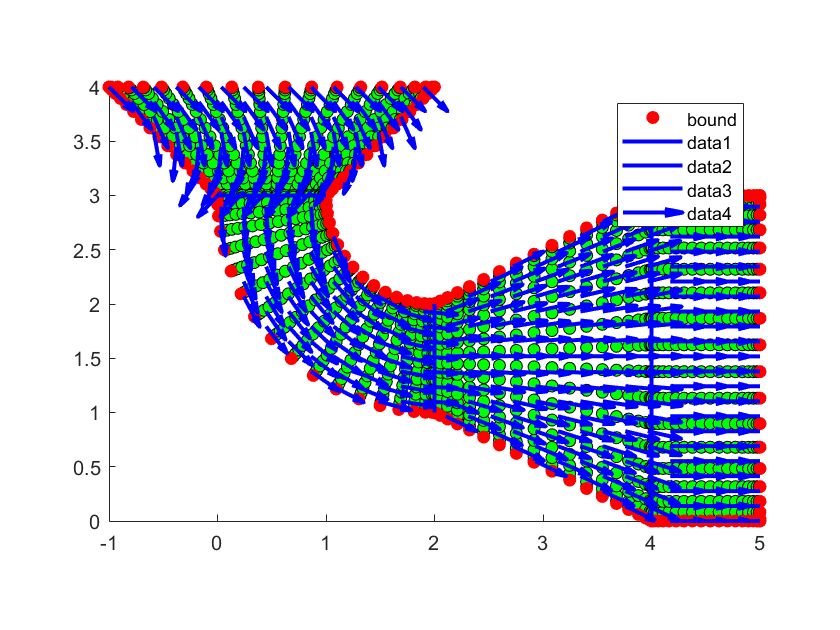
\includegraphics[scale=0.35]{F1.png}
%%		\caption{Forward $\rho$ for $a = 0.01$} 
%%		\label{F1}
%%	\end{figure}
%
%\begin{document}

\section{2DChebClass implementation for different shapes}	
\subsection{The interval (1D)}
In order to construct a line in the 2DChebClass library, three inputs have to be given; the endpoints of the interval and the number of discretization points $N+1$.
\subsubsection{Discretization points, boundaries, normals}
Pseudospectral methods on non-periodic domains are based on polynomial interpolation on non-equispaced points.  
Typically, Chebyshev points $\{x_j\}$, $j = 0,..,N$, are chosen as collocation points on $[-1,1]$, which are defined as:
\begin{align}\label{defChebyshevPoints}
	x_j= \cos\bigg(\frac{j \pi}{N}\bigg), \quad j=0,1,...,N,
\end{align}	
see \cite{bibTrefethen}.
These points are clustered at the endpoints of the interval, and sparse around $0$. Using this approach, the points are distributed from $1$ to $-1$, which is counter-intuitive. Therefore, in the code library 2DChebClass \cite{GoddardPseudospectralCode1}, which is used in producing the results of this report, the Chebyshev points are automatically flipped back to run from $-1$ to $1$. All computations in 2DChebClass are done on this computational domain $[-1,1]$. A vector $\vec x$ on $[-1,1]$ can then be mapped onto a physical domain $[a,b]$ of interest via the following linear map
\begin{align}\label{eq:linearmap}
\vec y = a + \frac{(\vec x+1)(b-a)}{2}.  
\end{align}
The inverse map is 
\begin{align}\label{eq:invlinearmap}
\vec x = -1 + \frac{2(\vec y-a)}{b-a}.
\end{align}
\\
The boundary of the domain is found by creating a vector of size $N$, which contains ones at the boundary points (i.e. $x_{min}$ and $x_{max}$) and zeros everywhere else. Note that the boundary points are found by evaluating the computational minimum and maximum, rather than the physical one.
The normal vectors for the line are simply defined as the one dimensional outward normals $n_1 = -1$, located at $y_{min}$ and $n_2 = 1$ at $y_{max}$. 
\subsubsection{Interpolation}\label{sec:1DInterp}
A function of interest, $f$, is evaluated at the Chebyshev points $\{x_j\}$ and a grid function, $f_j := f(x_j)$, is defined. There exists a unique polynomial of degree $\leq N$ that can be used to interpolate a function $f$ on the grid points $x_j$. The polynomial $p_N$ satisfies, by definition, the following relationship
\begin{align}\label{eqnptov1}
	p_N(x_j)=f_j,
\end{align}
so that the residual $p_N(x_j) -f_j$ is zero at these points. Therefore, this method is called a collocation method, see \cite{Boyd1}. Interpolation on the Chebyshev grid is done using barycentric Lagrange interpolation, derived in \cite{bibTrefethenBerrut1}. The barycentric formula is
\begin{align*}
	p_N(x)= \frac{\displaystyle \sum_{k=0}^N \frac{\tilde w_j}{x-x_j}f(x_j)}{\displaystyle \sum_{j=0}^N \frac{\tilde w_j}{x-x_j}},
\end{align*}
where the weights are defined as
\begin{align*}
	\tilde w_j = (-1)^j d_j, \quad d_j = 
	\left \{
	\begin{tabular}{c}
		$\frac{1}{2}$ \text{for} $j=0$, $j=N$, \\
		$1$ \text{otherwise}, \phantom{abksla} 
	\end{tabular}
	\right .
\end{align*}
see \cite{bibTrefethenBerrut1} and \cite{GoddardPseudospectralCode1}. In the code library 2DChebClass, this is implemented as a matrix-vector product, interpolating from the set of points $\{x_j\}$, onto another set of points $\{x_i\}$, where $i = 0,...., M$ and $j = 0, ...., N$.  The interpolation matrix is of the form
\begin{align*}
	\text{Interp}_{ij} = \frac{1}{\omega_i} \left(\frac{\tilde w_j}{x_i-x_j}\right), \qquad \omega_i = \displaystyle \sum_{k=0}^N \frac{\tilde w_k}{x_i-x_k}.
\end{align*} 
Generally, the set $\{x_j\}$ lies in computational space $[-1,1]$, while the second set of points can be customised by the user, to be any $M$ points in $[-1,1]$. There is another function in 2DChebClass, which takes a set of $M$ points $\{x_j\}$ in physical space as the set to be interpolated onto. This set of points is then first mapped onto the computational domain, using a linear map, before the interpolation matrix is computed, as described above. This method can then be applied to interpolating an arbitrary set of values $\{f_j\}$ onto the new set of points $\{f_i\}$. 
\subsubsection{Differentiation} \label{sec:1DDiff}
The derivation of the Chebyshev differentiation matrices is described below, following the presentation in \cite{bibTrefethen}. Given a polynomial $p_N$ (++definitely same as above??++), where condition \eqref{eqnptov1} holds, it can be differentiated so that $f'_j = p_N'(x_j)$, which can be rewritten as a multiplication of $f_j$ by a $(N+1) \times (N+1)$ matrix, denoted by $D$, as follows
\begin{align*}
	f'_j= D f_j,
\end{align*}
using (\ref{eqnptov1}).
A $(N+1) \times (N+1)$ differentiation matrix $D$ has the following entries, compare with \cite{bibTrefethen}
\begin{align*}
	(D)_{00}&= \frac{2N^2 +1}{6},\\
	(D)_{NN}&= -\frac{2N^2 +1}{6},\\
	(D)_{jj}&= -\frac{x_j}{2(1-x_j^2)}, \quad j=1,...,N-1,\\
	(D)_{ij}&= \frac{c_i}{c_j} \frac{(-1)^{i+j}}{(x_i-x_j)}, \quad i \neq j, \quad i,j=0,...,N,
\end{align*} 	
where 
\begin{align*}
	c_i =\left\{\begin{array}{l} 2, \quad i=0 \text{   or   }N, \\1, \quad \text{otherwise.}\end{array}\right.
\end{align*}	
The second derivative is represented by the second differentiation matrix $D_2$, which can be found by squaring the first differentiation matrix; $D_2=D^2$, and more generally the $j^{th}$ differentiation matrix $D_j$ is defined to be
\begin{align*}
	D_j=D^j.
\end{align*}
However, in \cite{GoddardPseudospectralCode1}, the exact coefficients, derived in a similar way as above for $D$, are used to compute $D_2$, since it is more accurate than squaring $D$. Furthermore, all differentiation matrices are derived in computational space and then mapped to physical space using the Jacobian transformation of the linear map \eqref{eq:linearmap}, which is defined to be
\begin{align}\label{eq:1DJacobian}
	J = \text{diag}\left(\tilde J \right), \quad \tilde J_j = \frac{d y_j}{d x_j}, \quad j = 0,...,N.
\end{align}
Then the physical differentiation matrix $D_y$ is defined as
\begin{align*}
	D_y = JD.
\end{align*}
Higher order differentiation matrices are mapped to physical space in a similar manner.
\subsubsection{Integration}\label{sec:1DInt}
In order to evaluate integrals in a similar way, the so-called Clenshaw--Curtis quadrature is used, which is derived in \cite{ClenCurt1}.
This is, for the integral over a smooth function $f$:
\begin{align}\label{eqnClenCurtQuad}
	\int_{-1}^1 f(x)dx = \sum_{j=0}^N w_jf(x_j),
\end{align}
where the weights are defined as:
\begin{align*}
	w_j = \frac{2d_j}{N}
	\left \{
	\begin{tabular}{c}
		$1- \displaystyle \sum_{k=1}^{(N-2)/2} \frac{2 \cos(2kt_j)}{4k^2-1} - \frac{\cos(\pi j)}{N^2 -1} \quad \quad\text{for $N$ even}$,\\
		$1- \displaystyle \sum_{k=1}^{(N-2)/2} \frac{2 \cos(2kt_j)}{4k^2-1} \quad \quad \quad \quad \quad \quad \ \ \ \text{for $N$ odd}$,
	\end{tabular}
	\right .
\end{align*}
see \cite{GoddardPseudospectralCode1}. In 2DChebClass this is implemented as a vector, such that $(\text{Int})_j = w_j$. Again, this is done in computational space, so that we multiply Int pointwise with the transposed Jacobian transformation \eqref{eq:1DJacobian} to map onto a desired physical domain, so that
\begin{align*}
	\left(\text{Int}_{\text{phys}}\right)_j = \text{Int}_j \tilde J_j.
\end{align*}
The integration vector can then be applied to a vector of function values $f_j$.
\subsubsection{Convolution}\label{sec:1DConv}
The final aspect to be considered is the convolution matrix, which is needed to compute convolution integrals. 
The convolution integral is defined as:
\begin{align*}
	\left(n \star \chi \right) (\vec y) = \int \chi ( \vec y - \vec{ z}) n (\vec{z}) d \vec{z},
\end{align*}
for a density $n$ and a weight function $\chi$.
A convolution matrix Conv can be created as follows
\begin{align*}
	\text{Conv}_{i,j} = \text{Int}_j \ \ \chi( y_i -  y_j)
\end{align*}
where $\vec y$ is the vector of physical points in $[a,b]$.
 The convolution integral is now defined as matrix vector multiplication, by applying the matrix Conv to a density vector $n$. The convolution matrix can be applied to different densities $n$, which saves computational time. 



\subsection{The quadrilateral (2D)}
In order to construct a quadrilateral in 2DChebClass, the set of vertices $\{X_i\} = \{(x_1^i,x_2^i)\}$, $i = 1,2,3,4$ has to be provided, as well as the number of discretization points in each direction, $N_1$ and $N_2$, has to be specified.
\subsubsection{Discretization points and domains}
In order to extend the one dimensional considerations to two-dimensional grids, a so-called tensor product grid has to be defined. First, Chebyshev points $x_1^j$, for $j=0,...,N_1-1$, on the $x$-axis and another set of Chebyshev points $x_2^i$, for $i=0,...,N_2-1$ on the $y$-axis are taken, both between $[-1,1]$. 
Then the following two so called Kronecker vectors are defined:
\begin{align}\label{eq:KroneckerVec}
	\mathbf{x}_1^{K}&=(x_1^0,x_1^0,...,x_1^0,x_1^1,x_1^1,...,x_1^1,...,x_1^n,x_1^n,...,x_1^n)^T,\\
	\mathbf{x}_2^{K}&=(x_2^0,x_2^1,...,x_2^m,x_2^0,x_2^1...,x_2^m,.....,x_2^1,x_2^2,...,x_2^m)^T,\notag
\end{align} 
where $n = N_1 - 1$ and $m = N_2 -1$.
In $\mathbf{x}_1^{K}$, each $x_1^j$ is repeated $N_2$ times, while $\mathbf{x}_2^{K}$, each sequence $x_2^0,x_2^1,...,x_2^m$ is repeated $N_1$ times. The total length of each vector is $N_1 \times N_2$. 
These vectors are defined, so that the set $(\mathbf{x}_1^{K},\mathbf{x}_2^{K})$ is a full set of all Chebyshev points on the two-dimensional tensor grid in computational space. An equivalent set can be defined for the points on the physical domain. Note that the points are clustered around the boundary of the two-dimensional grid and sparse in the middle of the grid.
\\
\\
As in the one dimensional case we can map the points $(\mathbf{x}_1^{K},\mathbf{x}_2^{K})$ to an arbitrary quadrilateral shape discretized via $(\mathbf{y}_1^{K},\mathbf{y}_2^{K})$. We use the superscript $k$ to indicate that $x^k \in \mathbf{x}^{K}$, for $k = 0,1,....,(N_1 - 1)\times (N_2 - 1)$. We first apply a linear map from $[-1,1]^2$ to $[0,1]^2$ 
\begin{align*}
	x_1^k = \frac{x_1^k+1}{2}, \quad
	x_2^k = \frac{x_2^k+1}{2}.
\end{align*}
Then the bilinear maps
\begin{align}\label{eq:bilinear1}
	y_1^k &= \alpha_1 + \alpha_2 x_1^k + \alpha_3 x_2^k + \alpha_4 x_1^k x_2^k,\\
	y_2^k &= \beta_1 + \beta_2 x_1^k + \beta_3 x_2^k + \beta_4 x_1^k x_2^k, \notag
\end{align}
take the points on the computational domain to the ones on the physical domain. The $\alpha_i$, $\beta_i$ are determined by mapping the coordinates of the four corners of the computational domain in a cyclic order onto the corners of the quadrilateral. 
The Jacobian of this bilinear map is also saved in this step, as well as the Hessians with respect to both variables.
However, most of the time we are given the coordinates of the quadrilateral in physical space, so that we have to map back to the computational domain. In order to do this, we again need to first find the values of the parameters $\alpha_i$ and $\beta_i$ and then invert the bilinear map to solve for the set of points on the computational domain.
We define a matrix B, with $A = BY$, such that $A_i = (\alpha_i, \beta_i)$, where $i = 1,2,3,4$, based on the bilinear maps \eqref{eq:bilinear1}, as
\begin{align*}
	B  =
	\begin{pmatrix}
		1 & 0 & 0 & 0 \\
		- 1 & 1 & 0 & 0 \\
		-1 & 0 & 0 & 1 \\
		1 & -1 & 1 & -1
	\end{pmatrix}	.
\end{align*}
Once we know the values of the parameters, we can solve the inverse map
\begin{align*}
	x_1^k = \frac{y_1^k - \alpha_1 -\alpha_3 x_2^k}{\alpha_2 + \alpha_4 x_2^k}
\end{align*}
and the quadratic
\begin{align*}
	a&\left(x_2^k\right)^2 + bx + c = 0,\\
	a &= \alpha_4 \beta_3 - \alpha_3 \beta_4,\\
	b &= \alpha_4 \beta_1 - \alpha_1 \beta-4 + \alpha_2 \beta_3 -\alpha_3 \beta_2 + y_1^k \beta_4 - y_2^k \alpha_2,\\
	c &= \alpha_2 \beta_1 - \alpha_1 \beta_2 + y_1^k \beta_2 - y_2^k \alpha_2.
\end{align*}
These give us the values for the $x_1^k$ and $x_2^k$ on $[0,1]^2$. In order to map to the computational domain $[-1,1]^2$, we apply a final linear map
\begin{align*}
	x_1^k = 2x_1^k - 1 \quad	x_2^k = 2x_2^k - 1.
\end{align*}


\subsubsection{Boundaries and Normals}
We can define the boundary of the quadrilateral by defining vectors for each of the four sides of the quadrilateral as follows. We do this on the computational domain $[-1,1]^2$, since each of the sides of the computational domain is conformally mapped onto a corresponding side of the quadrilateral. It is then straightforward to define a boolean vector of size $N_1 \times N_2$, which contains ones where $x_1 == x_{1,min}$ and zeros everywhere else, to define the left boundary of the square. We can then do the same for the other sides. We combine these four vectors to one boundary vector of length $N_1 \times N_2$, which contains ones at each of the four faces and zeros everywhere else. 
\\
The normal vectors of the quadrilateral are found by considering the four corners of the shape. We have the four corners $\{Y_i\} = \{(y_1^i,y_2^i)\}$, starting from the left bottom corner and defined in clockwise order. We then have the following set of normals $n_l$, $n_r$, $n_t$, and $n_b$, for the left, right, top and bottom normal respectively.
For the left normal we first define the vector
\begin{align*}
     \vec m_l = \left(y_2^2 - y_2^1, y_1^2 - y_1^1 \right) := \left(m_{l,1},m_{l,2} \right). 
\end{align*}
We then define the normal to be
\begin{align*}
	\vec n_l =  \sgn (m_{l,1})\frac{\left(-m_{l,1},m_{l,2} \right)}{\sqrt{m_{l,1}^2+m_{l,2}^2 }},
\end{align*}
where the negative first component and $\sgn (m_{l,1})$ are taken so that we 
consider the outward normal. We furthermore want to work with the unit normal, which is the reason for the normalisation term. The other three normals are therefore defined as
\begin{align*}
	\vec n_r &=  \sgn (m_{r,1})\frac{\left(m_{r,1}, - m_{r,2} \right)}{||\vec m_{r} ||_{l_2}},\\
	\vec n_t &=  \sgn (m_{t,2})\frac{\left(-m_{t,1},m_{t,2} \right)}{||\vec m_{t} ||_{l_2}},\\
	\vec n_b &=  \sgn (m_{b,2})\frac{\left(m_{b,1},-m_{b,2} \right)}{||\vec m_{b} ||_{l_2}}.
\end{align*}
In each of these terms, the definition of the $m_1$ is the difference in $y_2$ components, where the top coordinate is subtracted from the bottom coordinate and the $m_2$ refer to the left $y_1$ value being subtracted from the right $y_1$ value.
Each of these normal vectors has values on its respective face of the quadrilateral and zeros everywhere else. We then combine these four vectors using the boundary boolean vector which we have defined in the above step. This means that the normals on the corners get summed together, since each of the two faces meeting at a corner has a normal defined at the corner. The normal at a corner is not uniquely defined. However, it is convenient to define it such that it is the average of the two normals from each shape. This is done by normalising the sum of the two normals, as demonstrated here for the corner normal between the left and top face of the quadrilateral
\begin{align*}
	\vec n_c = \frac{\left(\vec n_{l} + \vec n_{t} \right)}{||\vec n_{l} + \vec n_{t}  ||_{l_2}}.
\end{align*}

\subsubsection{Interpolation}\label{sec:2DQuadInterp}
Interpolation in two dimensions is based on the idea of Kronecker tensor products. The interpolation matrices $\text{Interp}_1$ and $\text{Interp}_2$ are computed for each set of points $\{x_1^j\}$ on the $x$-axis and $\{x_2^i\}$ in the $y$ direction, as explained in Section \ref{sec:1DInterp}. The Kronecker product of these two matrices is taken resulting in the two-dimensional interpolation matrix. For an example with $i = j = 0,1,2$, this is the block matrix of size $ 9 \times 9$
\begin{align*}
	\text{Interp} &= \text{Interp}_1 \otimes \text{Interp}_2 \\
	&= 
	\begin{pmatrix}
		\text{Interp}_1(0,0) \times \text{Interp}_2 & \text{Interp}_1(0,1) \times \text{Interp}_2& \text{Interp}_1(0,2)  \times \text{Interp}_2\\
		\text{Interp}_1(1,0)  \times \text{Interp}_2 & \text{Interp}_1(1,1) \times  \text{Interp}_2& \text{Interp}_1(1,2)  \times \text{Interp}_2\\
		\text{Interp}_1(2,0)  \times \text{Interp}_2 & \text{Interp}_1(2,1)  \times \text{Interp}_2& \text{Interp}_1(2,2)  \times \text{Interp}_2
	\end{pmatrix}.
\end{align*}
\subsubsection{Differentiation}
A similar approach, using Kronecker vectors, can be used to find the Chebyshev differentiation matrices for two-dimensional problems as follows, compare to \cite{bibTrefethen}. For a first derivative $D$ in the $x$ direction, a Kronecker product is taken of the one-dimensional Chebyshev differentiation matrix, which is computed as explained in Section \ref{sec:1DDiff}, with the identity, as demonstrated here with three points
\begin{align*}
	D_{x_1}&=I \otimes D = 
	\begin{pmatrix}
		1 & 0 & 0\\
		0 & 1 & 0 \\
		0 & 0 & 1
	\end{pmatrix}
	\otimes
	\begin{pmatrix}
		d_{11} & d_{12} & d_{13}\\
		d_{21} & d_{22} & d_{23} \\
		d_{31} & d_{32} & d_{33}
	\end{pmatrix}
	\\&=
	\begin{pmatrix}
		d_{11} & d_{12} & d_{13} & & &  & & &\\
		d_{21} & d_{22} & d_{23} & & & & & & \\
		d_{31} & d_{32} & d_{33} & & & & & & \\
		& & &d_{11} & d_{12} & d_{13} & & &\\
		& & &d_{21} & d_{22} & d_{23}  & & &\\
		& & &d_{31} & d_{32} & d_{33} & & &\\
		& & & & & &d_{11} & d_{12} & d_{13}\\
		& & & & & &d_{21} & d_{22} & d_{23}  \\
		& & & & & &d_{31} & d_{32} & d_{33} 
	\end{pmatrix},
\end{align*}
where the block structure matches the repetition of each $x_1^j$ in $\mathbf{x}_1^{K}$.
The second derivative with respect to ${x_1}$, $D_{x_1x_1}$ can be found equivalently by computing $D_{x_1x_1} = I \otimes D_2$, where $D_2$ is the second order differentiation matrix in one dimension, as explained in Section \ref{sec:1DDiff}. 
The derivative with respect to $y$ is found by taking the Kronecker product the other way around
\begin{align*}
	D_{x_2}&=D \otimes I = 
	\begin{pmatrix}
		d_{11} & d_{12} & d_{13}\\
		d_{21} & d_{22} & d_{23} \\
		d_{31} & d_{32} & d_{33}
	\end{pmatrix}
	\otimes
	\begin{pmatrix}
		1 & 0 & 0\\
		0 & 1 & 0 \\
		0 & 0 & 1
	\end{pmatrix}
	\\&=
	\begin{pmatrix}
		d_{11} & & & d_{12} & & & d_{13} & & \\
		& d_{11} & & & d_{12} & & &  d_{13} & \\
		& & d_{11} & & &  d_{12} &  & & d_{13}\\
		d_{21} & & & d_{22} & & & d_{23} & & \\
		& d_{21} & & & d_{22} & & &  d_{23} & \\
		& & d_{21} & & &  d_{22} &  & & d_{23}\\
		d_{31} & & & d_{32} & & & d_{33} & & \\
		& d_{31} & & & d_{32} & & &  d_{33} & \\
		& & d_{31} & & &  d_{32} &  & & d_{33}\\
	\end{pmatrix},
\end{align*}
which now matches the repetition of each $x_2^0,...x_2^m$ in $\mathbf{x}_2^{K}$.
We have the following operators for the quadrilaterals in computational space
\begin{align*}
	\Grad &= \left(D_{x_1}, D_{x_2}\right),\\
	\Div &=\left(D_{x_1}, D_{x_2}\right)^\top,\\
	\Lap &= D_{x_1x_1} + D_{x_2x_2}.
\end{align*}
We need to be map these to the physical domain. This is done by applying the Jacobian of the transformation between the physical and computational space to the differentiation matrix.
The Jacobian is defined as
\begin{align*}
	J = \begin{pmatrix}
		\frac{\partial \mathbf{y}_1^{K}}{\partial \mathbf{x}_1^{K}} & \frac{\partial \mathbf{y}_1^{K}}{\partial \mathbf{x}_2^{K}}\\
		\frac{\partial \mathbf{y}_2^{K}}{\partial \mathbf{x}_1^{K}} & \frac{\partial \mathbf{y}_2^{K}}{\partial \mathbf{x}_2^{K}}
	\end{pmatrix},
\end{align*}
however, each of these entries are  vectors, so that this becomes a three dimensional array. We compute $\tilde J = \left(J^\top\right)^{-1}$ and get the gradient operator 
\begin{align*}
	\Grad = \left( \text{diag}\left(\tilde J_{11}\right) D_{x_1} + \text{diag}\left(\tilde J_{12}\right) D_{x_2},\text{diag}\left(\tilde J_{21}\right) D_{x_1} + \text{diag}\left(\tilde J_{22}\right) D_{x_2}\right).
\end{align*}
The construction of the Laplacian follows in a similar manner, using the Hessian matrices of the bilinear map but is more complex in the computational implementation.


\subsubsection{Integration}\label{sec:2DQuadInt}
The two dimensional integration vector is found by considering the two integration vectors for the points in the $x$ and the $y$ axis directions. The Kronecker product of these are taken and then multiplied by the determinant of the Jacobian of the mapping to the physical domain, since the integration vectors are computed on the computational grid. This gives the two dimensional integration vector.

\subsubsection{Convolution}\label{sec:2DQuadConv}
The construction of the convolution matrix is identical to the one in one dimension, see Section \ref{sec:1DConv}, except that $\chi$ takes both $\mathbf{y}_1^{K}$ and $\mathbf{y}_2^{K}$ as inputs and the integration vector involved is the two dimensional integration vector.
We have
\begin{align*}
	\text{Conv}_{i,j} = \text{Int}_j \ \ \chi({y}_1^{i} - {y}_1^{j},{y}_2^{i} - {y}_2^{j}).
\end{align*}
If the function $\chi$ only takes one input, we  consider the two given differences of points 
\begin{align*}
	d_1^{i,j} = {y}_1^{i} - {y}_1^{j}, \quad
	d_2^{i,j} = {y}_2^{i} - {y}_2^{j},
\end{align*}
and compute the euclidean distance between $d_1$ and $d_2$ to get the convolution matrix
\begin{align*}
	\text{Conv}_{i,j} = \text{Int}_j \ \ \chi(||d_1^{i,j}, d_2^{i,j}||_{l_2}).
\end{align*}

\subsection{The wedge (2D)}
For a wedge, inner and outer radius, maximum and minimum angle as well as the origin of the wedge have to be given. Furthermore, the number of discretization points for each direction has to be given.
\subsubsection{Discretization points and domains}\label{sec:2DWedgePts}
A wedge is a section of an annulus, the boundary of which is defined in polar coordinates by an inner and outer radius $r$ as well as a minimum and maximum angle $\theta_1$ and $\theta_2$. While $\theta_1$ should be chosen to lie in $[0, 2 \pi]$, the coordinate $\theta_2$ is mapped into this principal domain by computing 
\begin{align*}
	\theta_2 = \theta_1 +  d, \quad \text{where} \quad d = \theta_2 - \theta_1\mod 2 \pi.
\end{align*}
The wedge can be conformally mapped to a computational domain $[-1,1]^2$ (in polar coordinates ?!). For this the Kronecker vectors \eqref{eq:KroneckerVec} for the computational points $\{x_1\}$ and $\{x_2\}$ are taken. 
The Kronecker points $\mathbf{x}_1^{K}$ and $\mathbf{x}_2^{K}$ can then be mapped to the physical domain in $r$ and $\theta$ using the linear map \eqref{eq:linearmap} and then back to the computational domain using the map \eqref{eq:invlinearmap} from the one dimensional code. The derivatives of the map \eqref{eq:linearmap} for both variables are stored in the Jacobian matrix $J$.


\subsubsection{Boundaries and normals}
The boundaries of this shape are found in an identical manner to the quadrilateral case, since this is based on the computational grid. The definition of the normals in polar coordinates is straightforward (+ explain+). On the side with $\theta = \theta_2$ and on $r = r_2$ we have that $\vec n = (1,0)$, $\vec n = (0,1)$ and on the boundaries where $\theta = \theta_1$ and on $r = r_1$, we get that $\vec n = (-1,0)$, $\vec n = (0,-1)$. Since these are added together to result in the full set of normals, the set of normals at the corners is $\{\vec n_c\} = \{(-1,-1), (-1,1), (1,-1), (1,1)\}$. 
\\
\\
It can be useful to compute the normals in Cartesian coordinates, for example for plotting or for multishape applications. For this we have to consider the four faces of the shape, the inner and outer radii $r_i$, $r_o$ and inner and outer angle $\theta_i$ and $\theta_o$.

For the outer radius, we get $m_{r2,1} = \text{diag}(1)$ and $m_{r2,2} = \text{diag} (\theta)$. Equivalently, for the side where $\theta_2$ is constant, we have $m_{2,1} = \text{diag}(1)$ and $m_{2,2} = \text{diag} (\theta) + \text{diag} (\pi/2)$. For the inner radius we get have $m_{r1,1} = \text{diag}(1)$ and $m_{r1,2} = \text{diag} (\theta) + \text{diag} (\pi)$. For the side where $\theta_1$ is constant we have $m_{t1,1} = \text{diag}(1)$ and $m_{t1,2} = \text{diag} (\theta) + \text{diag} (3\pi/2)$.
The first components of each normal, which correspond to the radial variable, $m_{r2,1}, \ m_{r1,1}, \ m_{t2,1}, \ m_{t1,1}$ are combined to $n_1$. Any points that do not lie on the boundary are deleted. 
For the second component of the normals, extra care has to be taken at the corners of the shape to fix the angles. The computation for each pair of angles is explained in Algorithm \ref{alg:WedgeNormalCart}.
Then all components $m_{r2,2}, \ m_{r1,2}, \ m_{t2,2}, \ m_{t1,2}$, with the update at the corners is stacked to give $n_2$ and any points that are not on the boundary are deleted.
We combine $n_1$ and $n_2$, apply the standard transformation from polar to Cartesian coordinates to get the normal vectors for the wedge in Cartesian coordinates.
\\
\begin{algorithm}[H]
	\SetAlgoLined
	Given two angles $\theta_1$ and $\theta_2$ at the corner of the wedge, we normalise to get a resulting angle $\theta_c$.
	Set $\phi = \theta_2 - \theta_1$\\
	\uIf{$\abs{\phi}\leq \pi$}{
		$\theta_c = \theta_1 + \phi/2$
	}\uElseIf{$\pi<\phi \text{ and } \phi<(3/2)\pi$}{
$\theta_c = \theta_1 + (2\pi-\phi)/2$}
\Else{$\theta_c = = \theta_1-(2\pi-\phi)/2$	}	
Set $ \theta_c = \theta_c \mod 2 \pi$.
	\caption{Determining angles of normals}
	\label{alg:WedgeNormalCart}
\end{algorithm}



\subsubsection{Interpolation and differentiation}
Since interpolation is done on the computational grid this is equivalent to the discussion in Section \ref{sec:2DQuadInterp}.
\\
\\
In order to derive the differentiation matrices for the wedge, we start with the one-dimensional differentiation matrices described in Section \ref{sec:1DDiff}. Since these are derived on the computational domain, we have to map them to the physical domain. This is done for each coordinate individually so that we have
\begin{align*}
	D_r = J_1D \otimes I \quad 	D_\theta =I \otimes J_2D,
\end{align*} 
where $D$ is the differentiation matrix for the one-dimensional domain and $J_1$ and $J_2$  are the corresponding Jacobians of the mapping from the computational to the physical domain. For each discretization point $j = 1,...,N$ we have $ J_1^j= \frac{dr^j}{dx_1^j}$ and $J_2^j = \frac{d\theta^j}{dx_2^j}$.
However, this will result in differentiation matrices with respect to the coordinates $r$ and $\theta$. In order to compute the gradient, divergence and Laplacian we have to use the standard definition of the polar versions to derive these. For $ r \neq 0$ we get
\begin{align*}
	\Grad  &= \left(D_r, \frac{1}{r} D_\theta\right) ,\\
	\Div &= \left(D_r + \frac{1}{r}, \frac{1}{r} D_\theta\right)^\top ,\\
	\Lap  &= D_{rr} +\frac{1}{r}D_r +  \frac{1}{r^2} D_{\theta \theta}.
\end{align*}
At $ r = 0$, we need to treat these operators more carefully. We know that $\frac{1}{r} D_\theta = D_{r\theta}$, since $D_\theta =0$ at $r = 0$, and so $ \Grad = \left(D_r, D_{r\theta}\right)$. Similarly, at $r = 0$, we get that $\Div = \left(2D_r, D_{r\theta}\right)^\top$. Finally we have that $\Lap = 2 D_{rr} + \frac{1}{2} D_{\theta\theta}D_{rr}$ at the origin.
These identities are derived by using L'Hopital's rule. In order to do this, we need to make some assumptions on the function $f$ we apply these matrices to. In particular, we assume that all derivatives in $\theta$ are zero, to get a smooth solution as we approach $r =0$. We can then apply L'Hopital's rule to to conclude that we have, for $f$ satisfying this condition, that $\displaystyle \lim_{r \to 0}\frac{1}{r} \frac{\partial f}{\partial \theta} = \lim_{r \to 0} \frac{\partial^2 f}{\partial r \partial \theta}$, since both the top and bottom of the fraction go to zero as $r \to 0$.

We furthermore assume that $f(0, \theta)=c$, where $c$ is an arbitrary constant, which again is an assumption which ensures that the solution is well defined at $r=0$, since otherwise the function would be multivalued, since $\theta$ is allowed to vary.
We can then conclude the following
\begin{align*}
	\lim_{r \to 0}\frac{f(r)}{r} = \lim_{r \to 0} \frac{f(r) - f(0)}{r} = \lim_{r \to 0} \frac{f(r) - c}{r} = \lim_{r \to 0} \frac{\partial f(r)}{\partial r},
\end{align*}
where the last equality follows from L'Hopital's rule.
\subsubsection{Integration and convolution}
The integration vector is found in the same way as discussed in Section \ref{sec:2DQuadInt}. However, since this is an integral in polar coordinates, in a last step the integration vector has to be multiplied pointwise by $r$ to satisfy the polar integration formula $\int \int f(r, \theta) r dr d\theta$.
\\
\\
The convolution matrix is computed in the same way as in Section \ref{sec:2DQuadConv}, now using the polar version of the integration vector. 
Note that the convolution we are computing is
\begin{align*}
	\left(n \star \tilde \chi \right) (r, \theta) = \int \int \tilde \chi (r - r', \theta - \theta') n (r',\theta') d r' d\theta',
\end{align*}
where $\tilde \chi$ is the polar version of the weight function $\chi$.
\subsection{The periodic box (2D)}
As in the case of the quadrilateral, the required inputs for a periodic box are the number of points in each direction $N_1$ and $N_2$, as well as the coordinates of the vertices. However, it is enough to provide $x_{1,\text{min}}$, $x_{2,\text{min}}$, $x_{1,\text{max}}$, $x_{2,\text{max}}$, since we consider a box.

\subsubsection{Domains, boundaries, normals}
The periodic box has the first coordinate in in Cartesian space, discretized with Chebyshev points, the second coordinate is in Fourier space, using an equispaced discretization with stepsize $h = 2\pi /N$. This coordinate $\vec x_2$ is periodic. 
This means that while for the first coordinate $\vec x_1$ the linear maps \eqref{eq:linearmap} and \eqref{eq:invlinearmap} are still used, for the second coordinate we have the map 
\begin{align*}
	\vec y = a + (b-a) \vec x, 
\end{align*}
from $[-1,1]$ to $[a,b]$ and the corresponding inverse map
\begin{align*}
   \vec x = \frac{\vec y- a}{b-a}.
\end{align*}
The Kronecker vectors are created in the same way as in the case for the wedge, see Section \ref{sec:2DWedgePts}.
\\
The boundary is defined by finding the boundaries of the computational domain, as described in \ref{sec:2DWedgePts}. The normals are defined equivalently to the ones in Section \ref{sec:2DWedgePts}, since the periodic box only needs the unit normals.

\subsubsection{Interpolation}
In order to construct the interpolation matrix for this problem, we need to consider the interpolation matrices for each coordinate and take the Kronecker product of them.
The interpolation matrix for $\vec x_1$ is constructed following the description for one-dimensional domains in Section \ref{sec:1DInterp}, using barycentric Lagrange interpolation.
However, the interpolation matrix for $\vec x_2$ is constructed using Discrete Fourier Transforms (DFT). The account below follows the work in \cite{bibTrefethen}.
The DFT formula is
\begin{align*}
	\hat v_k = h \sum_{j = 1}^{N} e^{-ikx_j} v_j, \quad k = - \frac{N}{2} + 1, ..., \frac{N}{2},
\end{align*}
with stepsize $h$, and the inverse transform is
\begin{align*}
	v_j = \frac{1}{2 \pi} \sum_{k = - N/2 +1}^{N/2} e^{i k x_j} \hat v_k, \quad j = 1, ..., N.
\end{align*}
This inverse transform is well equipped to act as an interpolant for polar functions on periodic grids with period $2\pi$, once a small adjustment is made. We need to define $\hat v_{-N/2} = \hat v_{N/2}$ and get the interpolant
\begin{align}\label{eq:FourierInterp}
	p(x) = \frac{1}{4 \pi} e^{- i N x/2} \hat v_{-N/2} + \frac{1}{4 \pi} e^{i N x/2} \hat v_{N/2} + \frac{1}{2 \pi} \sum_{k = - N/2 + 1}^{N/2 - 1} e^{i k x} \hat v_k, 
\end{align}
where $x \in [-\pi/h, \pi/h]$, $h = 2\pi /N$.
An equivalent definition of the interpolant is derived by considering the interpolant for the delta function, see \cite{bibTrefethen} for a derivation.
We get
\begin{align*}
	p(x) = \sum_{m = 1}^N v_m S_N(x -x_m), 
\end{align*}
where
\begin{align}\label{eq:PeriodicInterpolant}
	S_N(x) = \frac{\sin(\pi x /h)}{(2 \pi /h)\tan(x/2)}
\end{align}
The interpolation matrix for the periodic variable in the code is defined as
\begin{align*}
	\text{Interp}_{2} = \left[e^{2\pi i \vec {x}_2^{I} 0}, e^{2\pi i \vec {x}_2^{I} j_1}, \cos(2\pi \vec {x}_2^{I} M) ,e^{2\pi i \vec {x}_2^{I} j_2}\right],
\end{align*} 
where $j_1 = 1,..., M-1$, $j_2 = M + 1,..., N$ and $M = (N + 1) /2$ if $N$ is odd and $M = N /2$ if $N$ is even. Note that the cosine term results from combining the first two terms in \eqref{eq:FourierInterp}. The set $\vec {x}_2^{I}$ is the set of points on which the second coordinate is interpolated on.
The fast Fourier transform matrix is defined as
\begin{align*}
	\text{FFTM} = I \otimes F, \quad \text{where} \quad	\text{F}_{jk} =  e^{- 2 \pi i / N jk},
\end{align*}
where $j, k = 0,..., N -1$.
The interpolation matrix is then
\begin{align*}
	\text{Interp} = \Re\left(\left(\text{Interp}_{1} \otimes \text{Interp}_{2}\right) \text{FFTM}\right).
\end{align*}
(+++ match this section notation wise (indices, N etc.) once clear +++)

\subsubsection{Differentiation}
In order to derive the differentiation matrices for the periodic grid, we return to the periodic interpolant \eqref{eq:PeriodicInterpolant}. This can be differentiated to give 
\begin{align*}
	S'_N(x_j) =\left\{\begin{array}{l} 0, \phantom{(-1)^j \cot(j h /2)} \quad j \equiv 0  \mod N\\
	\frac{1}{2} (-1)^j \cot(j h /2), \quad j \not \equiv 0  \mod N.\end{array}\right.
\end{align*}
This gives one column of the differentiation matrix, which has Toeplitz structure and is created in the code as, see \cite{bibTrefethen}
\begin{align*}
	D_{x_2} = 2\pi
	\begin{pmatrix}
		0 & & &  & &  & &-\frac{1}{2} \cot(h /2) \\
		-\frac{1}{2} \cot(h /2)&  & & &  & &   &\frac{1}{2} \cot(h) \\
		\frac{1}{2} \cot(h)& &  & & &    & & -\frac{1}{2} \cot(3 h /2)\\
		-\frac{1}{2} \cot( 3 h /2) & & &   & &  & & \\
		&  & & &   & &  & \\
		& & & &  & & & \frac{1}{2} \cot(h /2)\\
		\frac{1}{2} \cot(h /2)& &  & &   &  & & 0\\
	\end{pmatrix}.
\end{align*}
The factor of $2\pi$ is there to map the matrix back onto the grid $[-1,1]$. 
For the first coordinate $x_1$, the differentiation matrix is derived on the Chebyshev grid, as in the one-dimensional example. The two differentiation matrices are each mapped onto the physical domain, using Jacobian transformations, as described in Section \ref{sec:1DDiff}. The appropriate Kronecker products of the resulting differentiation matrices in physical space are taken to create $\Grad, \Div$ and $\Lap$ for the periodic box. 


\subsubsection{Integration and convolution}
We use the Clenshaw-Curtis integration weight in the first coordinate, see Section \ref{sec:1DInt}. This is multiplied by the one-dimensional Jacobian to map these weights from the computational onto the physical domain. In the fourier domain however, the integration weights are just $1/N$. These are also multiplied by the corresponding one-dimensional Jacobian. The integration vector for the periodic box is then the Kronecker product of the two one-dimensional integration vectors.
\\
\\
The convolution matrix is constructed in the same way as in Section \ref{sec:2DQuadConv}. However, in the quadrilateral case we computed the function $\chi$ at $\left(\vec {y}_1^{i} - \vec {y}_1^{j}, \vec{y}_2^{i} - \vec {y}_2^{i} \right)$. In the periodic box however, we need to consider the distances of ${y}_1^{i} - {y}_1^{j}$ and ${y}_2^{i} - {y}_2^{j}$, and compute them in two different ways. For the Chebyshev coordinate, nothing changes and we set $d_1^{i,j} = {y}_1^{i} - {y}_1^{j}$. Since the second coordinate is periodic, the distance between each pair of points in the periodic direction needs to reflect this. We need to compute 
\begin{align*}	
	d_2^{i,j} = c^{i,j} - \frac{L}{2}, \quad \text{where} \quad c^{i,j} =  {y}_2^{i} - {y}_2^{j} + \frac{L}{2} \mod L,
\end{align*}
and $L = y_2^{max} - y_2^{min}$. 
Then convolution matrix is
\begin{align*}
	\text{Conv}_{i,j} = \text{Int}_j \ \ \chi(d_1^{i,j}, d_2^{i,j}),
\end{align*}
where $\text{Int}$ is the integration vector for the periodic box.
If the function $\chi$ only takes one input, we take the euclidean distance between $d_1$ and $d_2$ and compute
\begin{align*}
	\text{Conv}_{i,j} = \text{Int}_j \ \ \chi(||d_1^{i,j}, d_2^{i,j}||_{l_2}).
\end{align*}
\subsection{Solving the PDE}
Regardless of the shape, the PDE can be solved as follows.
The initial condition $f_0$ of the PDE is discretized using Chebyshev points, or in the case of the periodic box, also equispaced points. The PDE is discretized using the derived differentiation and convolution matrices to give a vector $\text{dfdt}$ of size $N$ in one dimension and $N_1\times N_2$ in two dimensions, which is the discretized version of $\partial_t f$. The boundary conditions of the PDE are applied by replacing the boundary points of $\text{dfdt}$ with an algebraic equation for the boundary condition, i.e. by computing 
\begin{align*}
	\text{dfdt} \text{(boundary)} = \text{BC equation}.
\end{align*}
The mass matrix for this method is the identity matrix, denoted by M. At the boundary, we set M(boundary) = 0. 
Using an algebraic-differential equation solver, such as \texttt{ode15s} in Matlab, we solve M $\text{dfdt}$, so that on the boundary we solve BC equation = 0.
\section{Convergence Stuff}
+++++++++++++++ More on convergence stuff... see Boyd +++++++++++++++++++++++
The advantage of Spectral Methods is that, for smooth functions, the convergence is exponential, see \cite{Boyd1}:
\begin{align*}
	\text{Pseudospectral Error} \approxeq O \bigg[ \bigg( \frac{1}{N} \bigg)^N \bigg].
\end{align*}


A good overview on spectral methods is given in \cite{bibTrefethen} and a more in depth discussion can be found in \cite{Boyd1}.


\section{Implementation for multishape}
In the previous section we have discussed the implementation of the methods for different single shapes. While 2DChebClass supports solutions to PDEs on various single shapes, the method is now extended to compute the solution to a PDE on a multishape. A multishape is a complex domain, which is not fully described by one of the single shapes introduced in the previous section. However, it is possible to discretize the multishape domain in such a way that each of the elements is either a quadrilateral or a wedge. While that does not include all possible complex shapes, it does describe most physically relevant domains. The philosophy of this multishape code is to use the existing code library \cite{GoddardPseudospectralCode1}, which is designed to efficiently and accurately solve PDEs on individual shapes, to do the same on a multishape with minimal additional effort for the user.
\\
\\
The solution of a PDE on such a multishape domain is achieved by employing the spectral element method (SEM), since the multishape is discretized into elements. This method is similar in spirit to the finite element method (FEM). FEM discretizes a domain into elements and computes the solution to a given PDE on each of those elements and matches the solution at the boundaries. Expansions of basis functions are used, which are low order polynomials, for interpolation on an equispaced grid. SEM follows the same philosophy but uses higher order basis functions such as Chebyshev or Lagrange polynomials and Chebyshev-Lobatto points on an interpolation grid on each element, as opposed to an equispaced grid, to avoid the Runge phenomenon. At the intersections between the elements, $C^0$ continuity is enforced, by imposing two matching conditions, usually the solution and the first derivative, see \cite{Boyd1}. SEM was first introduced by Patera \cite{SEMPatera84} using  Chebyshev polynomials as basis functions and later adapted to Lagrange polynomials by Komatitsch and Vilotte \cite{SEMLagrange98}, which is now the standard choice \cite{Boyd1}.
While this method is widely used to solve PDEs in their weak form, in this work the strong form of the PDE is considered, since this aligns best with the existing framework. Furthermore, instead of matching the first derivative of the solution at the intersection of two elements, the flux is matched. 


\subsection{Setting up the multishape}
In order to set up a multishape, each of the discretized elements have to be specified. The information that has to be given for each element is the number of discretization points, $N_1$ in the $x$-direction, $N_2$ in the $y$-direction, whether the element is a quadrilateral or a wedge and whether to match the internal boundaries between elements. Note that, in order to create a functioning multishape, the number of points of the neighbouring faces of two elements have to match. For a quadrilateral, the four coordinates of the edges have do be given. For a wedge, inner and outer radius, maximum and minimum angle as well as the origin of the wedge have to be given. 
As done throughout in the code, the main idea is to stack the vectors of the individual elements to result into a long vector of size $M \times 1$, where $M = \sum_i N^i_1 N^i_2$, where $i$ counts the number of elements in the multishape. An equivalent approach is taken for matrices. This stacking results in computations being done directly on the multishape, instead of individually on each element. (++ improve explanation ++)
\\
\\
Once this information is given, the vectors of computational points $\mathbf x_1^M$, $\mathbf x_2^M$ and physical points $\mathbf y_1^M$, $\mathbf y_2^M$ on the whole multishape can be set up. This is done as described in Algorithm \ref{alg:msPts}.
 One important thing to notice is that the vectors $\mathbf y_1^M$, $\mathbf y_2^M$ are now defined in Cartesian coordinates, even if some of the underlying shapes are wedges, for which polar coordinates are the natural choice.
 \\

\begin{algorithm}[H]	\label{alg:msPts}
	\SetAlgoLined
	\For{ishape in multishape}{
		\begin{itemize}
			\item Get computational points $\mathbf x_1^i$, $\mathbf x_2^i$ and physical points $\mathbf y_1^i$, $\mathbf y_2^i$.
			\item Add points to vector containing multishape points:
			\begin{align*}
				\mathbf x_1^M = [\mathbf x_1^M; \mathbf x_1^i], \quad
				\mathbf x_2^M = [\mathbf x_2^M; \mathbf x_2^i], \quad
				\mathbf y_1^M = [\mathbf y_1^M; \mathbf y_1^i], \quad
				\mathbf y_2^M = [\mathbf y_2^M; \mathbf y_2^i].
			\end{align*} 
		\end{itemize}			
	}
\For{ishape in multishape}{
	\If{ishape is polar}{
		\begin{itemize}
		\item Convert polar $\mathbf y_1^i$, $\mathbf y_2^i$ to cartesian $\mathbf y_{1, \text{Cart}}^i$, $\mathbf y_{2, \text{Cart}}^i$.
		\item Replace in $\mathbf y_1^M$, $\mathbf y_2^M$:
		\begin{align*}
			\mathbf y_1^M(\text{ishape}) = \mathbf y_{1, \text{Cart}}^i, \quad \mathbf y	_2^M(\text{ishape}) = \mathbf y_{2, \text{Cart}}^i.
		\end{align*}
	\end{itemize}
	}
}
\caption{Multishape points}
\end{algorithm}

\subsection{Boundaries and intersections}
In order to  determine the points that lie on the boundary of a multishape, we first have to determine which faces of which shapes intersect. Once we have this information, we can take the boundaries of the individual shapes and substract the intersection boundaries from these to get the multishape boundary.
The intersections between shapes are found by the code automatically, as explained in Algorithm \ref{alg:msIntersections}. We iterate through all pairs of shapes to check whether any of their faces intersect by comparing the points of each shape on these faces. One thing to note is that we also have to check whether the points on face $i$ are equal to the flipped vector of points on face $j$. This is to account for the fact that there are different ways of constructing these points on each shape.
Having found the intersections between the shapes, the boundary of the multishape is defined by a boolean vector of size $M$, containing ones at the boundary and zeros everywhere else, as in the case for single shapes. Algorithm \ref{alg:msBoundary} explains the steps.

\begin{algorithm}[H]
	\SetAlgoLined
	\For{ishape in multishape}{
		\For{jshape in multishape}{		
			\For{iface in ishape}{
				\For{jface in jshape}{
					\uIf{$Pts_{\text{iface}} == Pts_{\text{jface}}$}{
						\begin{align*}
							&\text{Intersections(ishape,jshape).Pts} = \text{Pts}_{\text{iface}}\\
							&\text{Intersections(ishape,jshape).Face} = \text{iface}\\
							&\text{Intersections(ishape,jshape).Corners} = \text{Corners}_{\text{iface}}\\
							&\text{Intersections(ishape,jshape).Flip} = \text{False}
						\end{align*}
					}
					\ElseIf{iface $==$ flip(jface)} 
					{
						\begin{align*}
							&\text{Intersections(ishape,jshape).Pts} = \text{Pts}_{\text{iface}}\\
							&\text{Intersections(ishape,jshape).Face} = \text{iface}\\
							&\text{Intersections(ishape,jshape).Corners} = \text{Corners}_{\text{iface}}\\
							&\text{Intersections(ishape,jshape).Flip} = \text{True}
						\end{align*}
					}
	}}}	}	
	\caption{Determining intersections between shapes in a multishape}
	\label{alg:msIntersections}
\end{algorithm}
\pagebreak
\begin{algorithm}[H]
	\SetAlgoLined
	\For{ishape in multishape}{
			\For{iface in ishape}{
				\For{jface in ishape}{
					\If{Intersections(ishape, jshape).Face = iface}{
						Set IntersectionTest(iface) = True\;
					}
				}
			\If{IntersectionTest(iface) = False}{
				Set Boundary(iface) = True\;
			}
	}	}	
	\caption{Determining the boundary of a multishape}
	\label{alg:msBoundary}
\end{algorithm}

Constructing the normal vector for the multishape is quite complex and explained in Algorithm \ref{alg:msnormals}. One thing to be mindful of is the change from polar to Cartesian coordinates and back. The final normal vector contains polar values when corresponding to a wedge element and Cartesian coordinates for quadrilateral elements of the multishape. Extra care has to be taken at the corners of the boundary where two shapes intersect. There the normals are averaged as explained in Algorithm \ref{alg:msnormals}. However, when the discretization of the multishape is more complex, this may sometimes not be sufficient, and the resulting outward normal is not sensible. For this reason it is possible to override any of the normals manually as a user. The effect is demonstrated in the validation tests in Section +++ ref validation tests +++.
\\
\begin{algorithm}[H]
	\SetAlgoLined
	\For{ishape in multishape}{
		\begin{itemize}
			\item Get normal vector inormal for ishape.
			\item Set normalVec(ishape) = inormal.
		\end{itemize}
		\uIf{ishape is polar}{
			\begin{itemize}
				\item 	Get Cartesian normal vector inormalCart for ishape.
				\item	Set normalCart(ishape) = inormalCart.
			\end{itemize}
		}\Else{
			\begin{itemize}
				\item Set	normalCart(ishape) = inormal.
			\end{itemize}
		}
	\begin{itemize}
		\item Delete entries that do not lie on the boundary of the multishape.
	\end{itemize}
	}
	
	Fixing normals at corners. Find entries in normalCart that share same points (up to a tolerance). Store points in duplicates. \\
		\For{dup in duplicates}{
			\uIf{override is True}{
			Normal vector $n$ at dup is specified by the user.
		}
		\Else{
			Average and normalize normals in normalCart(dup) to get $n$.
		}
		}
	Set normalCart(dup)$ = n $. \\
	 \For{ishape in multishape}{
	 	\uIf{ishape is polar}{
	 		Convert normals from normalCart(ishape) to polar coordinates and assign to normal(ishape).	
	 	}\Else{Set
	 	normal(ishape) = normalCart(ishape).
 	}
	 }
		
	\caption{Determining the outward normals of a multishape}
	\label{alg:msnormals}
\end{algorithm}


\subsection{Interpolation, differentiation, integration and convolution}
The interpolation matrix for the multishape is constructed by computing the individual interpolation matrices on each shape and stacking them together in a blockdiagonal matrix. The gradient, divergence and Laplacian operators for the multishape are constructed in an equivalent way. The integration vector is constructed by simply stacking the integration vectors for each shape. Each of these constructions is demonstrated in Algorithm \ref{alg:msinterp}.

\begin{algorithm}[H]
	\SetAlgoLined
	\For{ishape in multishape}{
		\begin{itemize}
			\item Get
			$\text{Interp}_{\text{ishape}}$,  $\Grad_{\text{ishape}}$,  $\Div_{\text{ishape}}$, $\Lap_{\text{ishape}}$, $\text{Int}_{\text{ishape}}$.
			\item Set \\
			Interp $=$ blkdiag(Interp, $\text{Interp}_{\text{ishape}}$),\\
			$\Grad =$ blkdiag(Interp, $\Grad_{\text{ishape}}$),\\
			$\Div =$ blkdiag(Interp, $\Div_{\text{ishape}}$),\\
			$\Lap =$ blkdiag(Interp, $\Lap_{\text{ishape}}$),\\
			Int $=$ (Int, $\text{Int}_{\text{ishape}}$).	
		\end{itemize}
		}	
	\caption{Constructing the interpolation matrix, gradient, divergence and Laplacian as well as the integration vector}
	\label{alg:msinterp}
\end{algorithm}
While computing the standard interpolation matrix is straightforward, computing the interpolation matrix for a set of physical points in multishape is a bit more complex.
Given a set of points $\mathbf{y}_1^I$ and $\mathbf{y}_2^I$ that we want to interpolate onto, we need to first determine which of these points are in which shape, since the interpolation is done shapewise as explained in Algorithm \ref{alg:msinterp}. Algorithm \ref{alg:msinterpPhys} illustrates this. (+++ check algorithm after meeting +++)

\begin{algorithm}[H]
	\SetAlgoLined
	\For{ishape in multishape}{
		Get $\mathbf{y}_1^I$ and $\mathbf{y}_2^I$ to interpolate onto\;
		\For{ishape in multishape}{
			\begin{itemize}
				\item Get computational points $x_1$, $x_2$ for ishape.
				\item Get $x_{1,\text{min}} = \min(x_1) - 10^{-10}$, $x_{1,\text{max}} = \max(x_1) + 10^{-10}$, $x_{2,\text{min}} = \min(x_2) - 10^{-10}$, $x_{2,\text{max}} = \max(x_2) + 10^{-10}$.
			\end{itemize}
		\If{ishape is polar}
		{Get polar version of $\mathbf{y}_1^I$ and $\mathbf{y}_2^I$.
		}
		\begin{itemize}
			\item Transform $\mathbf{y}_1^I$ and $\mathbf{y}_2^I$ to $\mathbf{x}_1^I$ and $\mathbf{x}_2^I$ in computational space, using the linear mapping associated to the shape.
			\item Define iMask = ($x_1>=x_{1,min}$) \& ($x_1<=x_{1,max}$) \& ($x_2>=x_{2,min}$) \& ($x_2<=x_{2,max}$) \& ~doneMask.
			\item Create new vectors that only contain the points of the shape:\\  $\mathbf{x}_1^I$(iMask), $\mathbf{x}_2^I$(iMask).
		\end{itemize}		
		\For{i in length($\mathbf{x}_1^I$(ishape))}{
			\begin{itemize}
				\item Compute interpolation matrix pointwise for $x_1(i) \in \mathbf{x}_1^I$(ishape), $x_2(i) \in \mathbf{x}_1^I$(ishape).
				\item Set Interp$_{\text{ishape}}$ = [ Interp$_{\text{ishape}}$, InterpolationMatrix($x_1(i), x_2(i)$)].
			\end{itemize}	
	}
		\begin{itemize}
			\item Stack interpolation matrices in a blockdiagonal:\\
			Interp $=$ blkdiag(Interp, $\text{Interp}_{\text{ishape}}$).
			\item Set doneMask(iMask) = True.
		\end{itemize}
	}
	\begin{itemize}
		\item Set Interp(~doneMask) = [].
		\item Set $\mathbf{y}_1^I$ = $\mathbf{y}_1^I$(doneMask), $\mathbf{y}_2^I$ = $\mathbf{y}_2^I$(doneMask).
	\end{itemize}
	}	
	\caption{Constructing the interpolation matrix for interpolating onto points in physical space}
	\label{alg:msinterpPhys}
\end{algorithm}

The convolution matrix cannot be taken from the individual shapes, since convolution is a global operation. We compute it in the exact same way as for a single quadrilateral, see Section \ref{sec:2DQuadConv}, now using the multishape points $\mathbf{y}_1^M$ and $\mathbf{y}_2^M$ and the integration vector that was constructed for the multishape.



\subsection{Boundary matching and solving the PDE}
As discussed above, the code automatically identifies the intersection boundaries between two shapes when setting up the multishape. Once the intersections between the neighboring shapes are identified, user-defined boundary conditions can be applied. There are currently two options, although the addition of further boundary conditions is straightforward. In general, both the solution to the PDE and the flux are matched at these intersection boundaries to create a coherent solution over the whole shape. Alternatively, hard walls between two shapes can be simulated easily, by applying a no-flux boundary condition at that intersection boundary. On boundaries which are on the outside of the multishape, the boundary conditions of the PDE, such as no-flux and Dirichlet conditions, can be applied in the same way as for single shapes.
The application of the boundary conditions and solution of the PDE follows the method for single shapes and is illustrated in Algorithm \ref{alg:msBCapplication}. Note that the mass matrix for a collocation method is diagonal. The boundary and matching conditions are applied by setting the relevant entries in the mass matrix to zero.
\\
	\begin{algorithm}[H]
		\SetAlgoLined
		\begin{itemize}
			\item Get discretized PDE $\text{dfdt}$.
			\item Get boundary condition equation BCeq and intersection boundary condition Intereq.
			\item Set the mass matrix M = diag(ones).
			\item Set M(boundary) = 0,  M(intersection) = 0.
			\item Set $\text{dfdt}$(boundary) = BCeq.
			\item Set $\text{dfdt}$(intersection)= Intereq.
			\item Compute M $\text{dfdt}$ using \texttt{ode15s}.
		\end{itemize}
		
		\caption{Applying boundary and intersection conditions, solving the PDE.}
		\label{alg:msBCapplication}
	\end{algorithm}
	
%	\pagebreak	
%	\bibliography{GeneralBib}
%	\bibliographystyle{unsrt}
	
%\end{document}